% !TeX spellcheck = en_GB

\section{\protect{\emoji{rocket}} Conclusion and future outlook}{

    \begin{frame}{\protect{\emoji{rocket}} Where did we came from, where do we go?}

        We talked about \texttt{CARSO} -- a novel framework devised to foil \textit{gradient-based adversarial attacks}, specifically targeted at image classification -- showing noteworthy improvements upon \texttt{IAT}, a strong contribution to \textit{off-manifold-to-on-manifold reprojection}, and solid \textit{innate robustness}.

        Experimental scope can be broadened, though:
        \begin{itemize}
            \item Proper, meticulous hyperparameter tuning;
            \item Different architectures;
            \item More complex datasets;
            \item Different \textit{media} (text, sequences, \etc\dots);
            \item Broader attack \textit{coverage} (e.g. against \textit{adaptive attacks});
            \item Comparison with additional defences.
        \end{itemize}

    \end{frame}

    \begin{frame}{\protect{\emoji{rocket}} Through \texttt{CARSO}, beyond \texttt{CARSO}}

        The work required to develop and assess \texttt{CARSO} evoked suggestions reaching far longer and broader than expected. Chiefly, in order of increasing conceptual distance...

        \begin{itemize}
            \item The idea that \textit{adaptive} defences may exist, explicitly steering their behaviour on the basis of the geometric properties of inputs or attacks faced. \texttt{CARSO} might even one (though embryonic, immature) of this kind.
            \item Weight-agnostic layers operating at the \textit{feature-specific} (or, traditionally, \textit{architecture/dataset-specific}) level -- able to produce \textit{zero-gradient} in expectation, without masking it.
            \item The possibility of informing the development (or... the \textit{training}?!) of \textit{deep learning} architectures with (the information contained in) neural activity recordings -- for the sake of one or the other, or both. And, why not: \textit{live-subject} recordings! \protect{\emoji{mouse}}
        \end{itemize}
    \end{frame}

    \begin{frame}{\protect{\emoji{rocket}} Hopefully part of a \textit{broader} endeavour... (I)}
        \centering
        \vspace*{10px}
        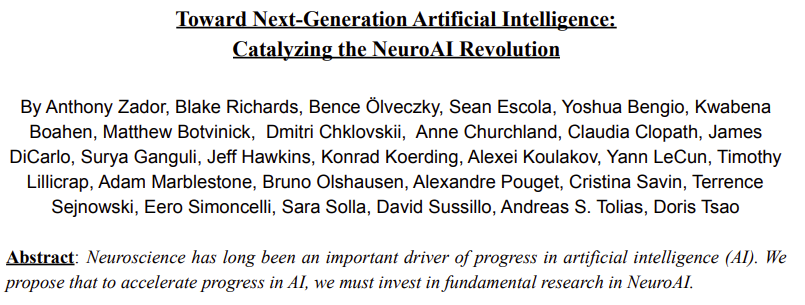
\includegraphics[width=0.98\textwidth, height=0.7\textheight, keepaspectratio]{towards_neuro_ai_paper_heading.png}
        \vspace*{10px}

        (Zador et al., 2022 -- \textit{ArXiv, abs/2210.08340})
        \vspace*{10px}
    \end{frame}

    \begin{frame}{\protect{\emoji{rocket}} Hopefully part of a \textit{broader} endeavour... (II)}
    \centering
    \vspace*{10px}
    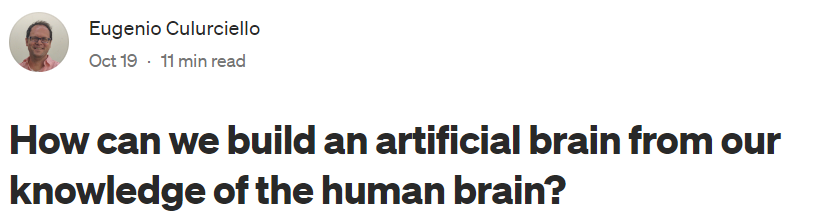
\includegraphics[width=0.98\textwidth, height=0.7\textheight, keepaspectratio]{culurciello_medium.png}
    \vspace*{10px}

    (Eugenio Culurciello, 2022 -- \textit{Medium.com}, see: {https://cutt.ly/culurciello\_brain\_2022})
    \vspace*{10px}
\end{frame}
}
